%tikz_draw
\documentclass[tikz, border=5, svgnames]{standalone}
\usepackage[utf8]{inputenc}
\usepackage[english]{babel}
\usepackage{amsmath}
\usepackage{amsfonts}
\usepackage{amssymb}
%tikzlibrary
\usetikzlibrary{arrows.meta}
%standalone preamble

\usepackage{pgfplots}
\begin{document}

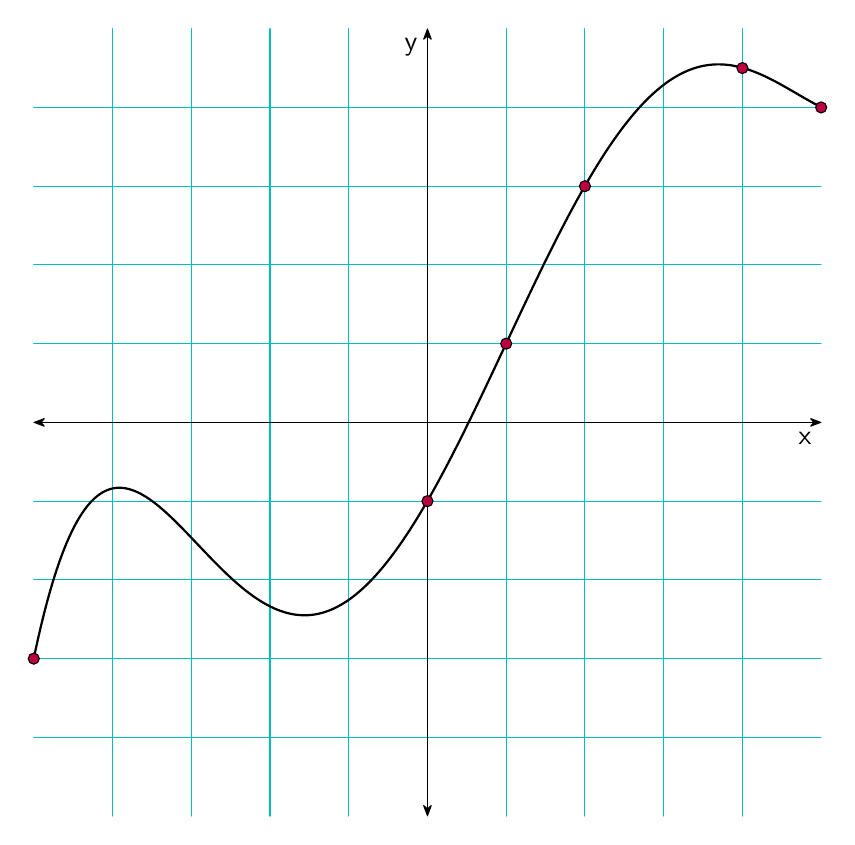
\begin{tikzpicture}

\foreach \i in {-4, -3, ..., 3, 4}
    \draw[line cap = round, Cyan!75!Black] (\i, -5) -- (\i, 5) (-5, \i) -- (5, \i);

\draw[{Stealth[round]}-{Stealth[round]}] (-5,0) -- (5,0);
\draw[{Stealth[round]}-{Stealth[round]}] (0, -5) -- (0,5);

\node at (5, 0) [anchor=north east] {$\mathsf{x}$};
\node at (0, 5) [anchor=north east] {$\mathsf{y}$};

\begin{axis}[axis x line=none,axis y line=none,xticklabels=\empty,yticklabels=\empty,xmin=-5, xmax=5,ymin=-5, ymax=5, xshift=-5cm, yshift=-5cm, x=1cm,  y=1cm]

\addplot [thick, line cap=round, samples=500, domain=-10:10] {0.00281746031746032*x^5 - 0.0129761904761905*x^4 - 0.111944444444445*x^3 + 0.384404761904762*x^2 + 1.73769841269841*x - 1};

\end{axis}

\filldraw[line width=0.4pt, fill=purple, draw=black, ] (1,1) circle (2pt);
\filldraw[line width=0.4pt, fill=purple, draw=black, ] (2,3) circle (2pt);
\filldraw[line width=0.4pt, fill=purple, draw=black, ] (0,-1) circle (2pt);
\filldraw[line width=0.4pt, fill=purple, draw=black, ] (5,4) circle (2pt);
\filldraw[line width=0.4pt, fill=purple, draw=black, ] (-5,-3) circle (2pt);
\filldraw[line width=0.4pt, fill=purple, draw=black, ] (4.0,4.5) circle (2pt);

\end{tikzpicture}
\end{document}
